% vim: set foldmethod=marker:
\documentclass[english]{article}

% {{{ Set Globals

\title{Advanced Databases}
\author{Itziar \\ Emilie}
\date{\today}

\newcommand{\uniClassInstructor}{Stanislav Vakaruk}
\newcommand{\uniClassDegree}{Software Engineering (Mention in Data Engineering)}
\newcommand{\uniClassYear}{3}
\newcommand{\uniClassSemester}{September 2025 - January 2026}
\newcommand{\uniClassCredits}{6}
\newcommand{\uniClassLanguage}{English}

% {{{ Basic stuff

%\author{Itziar Morales Rodríguez}
%\author{Author}

% Some basic packages
%\usepackage[utf8]{inputenc}
\usepackage[T1]{fontenc}
\usepackage[main=english]{babel}
\usepackage{graphicx}
\usepackage{float}
\usepackage{booktabs}
%\usepackage{lastpage}
%\usepackage{dirtytalk}
\usepackage{float}
%\usepackage{gensymb}

% Code
%\usepackage[cachedir=\detokenize{~/.cache/minted}]{minted}
\usepackage{listings}

% Use the Roboto font
%\usepackage[sfdefault,light]{roboto}
\renewcommand{\familydefault}{\sfdefault}
\usepackage{helvet}
% Set enumerate
%\usepackage{enumitem}
%\setlist{nosep}
%\setitemize{topsep=0.5em, itemsep=0.5em}
%\setenumerate{topsep=0.5em, itemsep=0.5em}
%\setitemize[1]{label=\bullet}
%\setitemize[2]{label=\circ}

% Adjust page margins
\usepackage{geometry} % Required for adjusting page dimensions and margins

\geometry{%
	paper=a4paper, % Change to letterpaper for US letter
	%total={209mm,157mm},
	top=3cm,% Top margin
	bottom=3cm,% Bottom margin
	left=2.5cm,% Left margin
	right=2.5cm, % Right margin
	headheight=30pt, % Header height
	footskip=1.4cm, % Space from the bottom margin to the baseline of the footer
	headsep=1.2cm, % Space from the top margin to the baseline of the header
	%showframe, % Uncomment to show how the type block is set on the page
}

% Don't indent paragraphs, leave some space between them
\usepackage{parskip}

% Floating elements
%\usepackage{wrapfig}

% Hide page number when page is empty
%\usepackage{emptypage}

\usepackage{caption}
\usepackage{subcaption}
\usepackage{multicol}
\usepackage[table,x11names]{xcolor}

% Hyper ref
\usepackage[
	pdfencoding=auto, psdextra, % Enable unicode and math in titles
	colorlinks=true,
	urlcolor=DodgerBlue4,
	linkcolor=DodgerBlue4,
	citecolor=DodgerBlue4
]{hyperref}
\PassOptionsToPackage{unicode}{hyperref}
\PassOptionsToPackage{naturalnames}{hyperref}
\pdfstringdefDisableCommands{\def\varepsilon{\textepsilon}}
\usepackage{bookmark}% faster updated bookmarks
%\usepackage{csquotes}

% Bibliography
% \usepackage[nottoc,numbib]{tocbibind} % add toc in index
%\usepackage[
%	autocite     = superscript,
%	backend      = biber,
%	sortcites    = true,
%	style        = numeric,
%	defernumbers = true
%]{biblatex}

% }}}

% {{{ Sectioning

%\usepackage{titlesec} % Required for modifying sections
\usepackage{tikz}

%------------------------------------------------
% Part

%\titleformat%
%{\part} % command
%[display] % shape
%{\bfseries\huge\scshape} % format
%{
%	\center%
%	Parte\ \thepart
%} % label
%{0.5ex} % sep
%{
%	\center
%} % before-code
%[
%	\vspace{-0.5ex}%
%] % after-code
%
%%------------------------------------------------
%% Chapter
%
%%\addto\captionsspanish{\renewcommand{\chaptername}{\assignmentChapterName}}
%%Options: Sonny, Lenny, Glenn, Conny, Rejne, Bjarne, Bjornstrup
%\titleformat%
%{\chapter} % command
%[hang] % shape
%{\LARGE\scshape} % format
%{\thechapter\ \ } % label
%{0.5ex} % sep
%{} % before-code
%[
%	\vspace{-0.5ex}%
%	\color{DodgerBlue3}\rule{\textwidth}{0.3pt}
%] % after-code
%
%\titlespacing{\chapter}{0pt}{-0.5cm}{1.5em}
%
%%------------------------------------------------
%% Section
%
%\titleformat%
%{\section} % command
%[hang] % shape
%{\bfseries\LARGE} % format
%{\thesection\ \ } % label
%{0.5ex} % sep
%{} % before-code
%[] % after-code
%
%
%%------------------------------------------------
%% SubSection
%
%\titleformat%
%{\subsection} % command
%[hang] % shape
%{\bfseries\Large} % format
%{\thesubsection\ \ } % label
%{0.5ex} % sep
%{} % before-code
%[] % after-code
%
%%------------------------------------------------
%% SubSubSection
%
%\titleformat%
%{\subsubsection}
%[hang]
%{\bfseries\large}
%{\thesubsubsection\ \ }
%{0.5ex}
%{}
%[]
%
%% }}}

% {{{ Math stuff

% Math stuff
\usepackage{amsmath}
\usepackage{amsfonts}
\usepackage{mathtools}
\usepackage{amsthm}
\usepackage{amssymb}
\usepackage{physics}

% Fancy script capitals
\usepackage{mathrsfs}
%\usepackage{cancel}

% Math code
%\usepackage{sagetex}

% Bold math
\usepackage{bm}

% Some shortcuts
\newcommand\N{\ensuremath{\mathbb{N} }}
\newcommand\M{\ensuremath{\mathfrak{M} }}
\newcommand\R{\ensuremath{\mathbb{R} }}
\newcommand\K{\ensuremath{\mathbb{K} }}
\newcommand\Z{\ensuremath{\mathbb{Z} }}
\renewcommand\O{\ensuremath{\emptyset}}
\newcommand\Q{\ensuremath{\mathbb{Q} }}
\newcommand\C{\ensuremath{\mathbb{C} }}
\newcommand\Dom{\ensuremath{\textrm{Dom}} }

% Add \contra symbol to denote contradiction
\usepackage{stmaryrd} % for \lightning
\newcommand\contra{\scalebox{1.5}{$\lightning$}}

% Theorem tools
\usepackage{thmtools}
%\usepackage{cleveref}

%\DeclareMathOperator{\sech}{sech}
%\DeclareMathOperator{\csch}{csch}
\DeclareMathOperator{\arccosh}{arcCosh}
\DeclareMathOperator{\arcsinh}{arcsinh}
\DeclareMathOperator{\arctanh}{arctanh}
\DeclareMathOperator{\arcsech}{arcsech}
\DeclareMathOperator{\arccsch}{arcCsch}
\DeclareMathOperator{\arccoth}{arcCoth}

%\newcommand\oast{\stackMath\mathbin{\stackinset{c}{0ex}{c}{0ex}{\ast}{\bigcirc}} }

% Theorems in fancy boxes
%\usepackage{todonotes}
%\usepackage[most]{tcolorbox}
%\tcbuselibrary{theorems}
%\tcbuselibrary{minted}
%\tcbset{listing engine=minted}

%\theoremstyle{definition}
%\newtheorem{definition}{Definition}[section]
%\newtcbtheorem[number within=section]{definition}{Definition}%
%{colback=green!5,colframe=green!35!black,fonttitle=\bfseries}{def}

\definecolor{codegreen}{rgb}{0,0.6,0}
\definecolor{codegray}{rgb}{0.5,0.5,0.5}
\definecolor{codepurple}{rgb}{0.58,0,0.82}
\definecolor{backcolour}{rgb}{0.95,0.95,0.92}

\lstdefinestyle{mystyle}{
	backgroundcolor=\color{backcolour},
	commentstyle=\color{codegreen},
	keywordstyle=\color{magenta},
	numberstyle=\tiny\color{codegray},
	stringstyle=\color{codepurple},
	basicstyle=\ttfamily\footnotesize,
	breakatwhitespace=false,
	breaklines=true,
	captionpos=b,
	keepspaces=true,
	numbers=left,
	numbersep=5pt,
	showspaces=false,
	showstringspaces=false,
	showtabs=false,
	tabsize=2
}

\lstset{style=mystyle}

%\newtcbinputlisting{\mathcodeinput}[3]{
%	listing engine=minted,
%	%minted style=colorful,
%	minted language={#2},
%	minted options={
%			fontsize=\small,
%			breaklines,
%			autogobble,
%			linenos,
%			numbersep=3mm,
%			mathescape=true
%		},
%	colback=DodgerBlue1!6,
%	colframe=DodgerBlue4,
%	boxrule=0.0mm,
%	left=5mm,
%	listing file={#1},
%	enhanced,
%	breakable,
%	overlay={
%			\begin{tcbclipinterior}
%				\fill[DodgerBlue2!20]
%				(frame.south west)rectangle([xshift=5mm]frame.north west);
%			\end{tcbclipinterior}
%		},
%	#3
%}

%\newtcblisting{mathcodebox}[2][]{
%	listing engine=minted,
%	%minted style=colorful,
%	minted language={#2},
%	minted options={
%			fontsize=\small,
%			breaklines,
%			autogobble,
%			linenos,
%			numbersep=3mm
%		},
%	colback=DodgerBlue1!6,
%	colframe=DodgerBlue4,
%	boxrule=0.0mm,
%	left=5mm,
%	enhanced,
%	breakable,
%	overlay={
%			\begin{tcbclipinterior}
%				\fill[DodgerBlue2!20]
%				(frame.south west)rectangle([xshift=5mm]frame.north west);
%			\end{tcbclipinterior}
%		},
%	#1
%}

% End example and intermezzo environments with a small diamond (just like proof
% environments end with a small square)
\usepackage{etoolbox}
%\AtEndEnvironment{eg}{\null\hfill$\qed$}%
\AtEndEnvironment{myproof}{\null\hfill$\square$}%

\newcommand{\exerciseSection}[1]{%
	\pagebreak
	\section*{#1}
	\addcontentsline{toc}{section}{\protect\numberline{}#1}%
}

%\usepackage{xifthen}

% Exercise
% Usage:
% \exercise{5}
% \subexercise{1}
% \subexercise{2}
% \subexercise{3}
% gives
% Problema 5
%   Problema 5.1
%   Problema 5.2
%   Problema 5.3
%\newcommand{\exercise}[1]{%
%  \problemDivider
%  \problem{#1}
%  \def\@exercise{#1}%
%}
%
%\newcommand{\subexercise}[1]{%
%  \problem{\@exercise.#1}
%}

% }}}

% {{{ Physics

\usepackage{physics}

% }}}

% {{{ Class stuff

% \lecture starts a new lecture (les in dutch)
%
% Usage:
% \lecture{1}{di 12 feb 2019 16:00}{Inleiding}
%
% This adds a section heading with the number / title of the lecture and a
% margin paragraph with the date.

% I use \dateparts here to hide the year (2019). This way, I can easily parse
% the date of each lecture unambiguously while still having a human-friendly
% short format printed to the pdf.

\def\testdateparts#1{\dateparts#1\relax}
\def\dateparts#1 #2 #3 #4 #5\relax{
	\marginpar{\small\textsf{\mbox{#1 #2 #3 #5}} }
}

\def\@lecture{}%
\newcommand{\lecture}[3]{
	\ifthenelse{\isempty{#3}}{%
		\def\@lecture{Class #1}%
	}{%
		\def\@lecture{Class #1: #3}%
	}%
	\subsection*{\@lecture}
	\marginpar{\small\textsf{\textbf{Class #1} \\ \mbox{#2}} }
}

\newcommand{\lectureMargin}[2]{
	\marginpar{\small\textsf{\textbf{Clase #1} \\ \mbox{#2}} }
}

\def\@studySession{}%
\newcommand{\studySession}[3]{
	\ifthenelse{\isempty{#3}}{%
		\def\@studySession{Study #1}%
	}{%
		\def\@studySession{Study #1: #3}%
	}%
	\subsection*{\@studySession}
	\marginpar{\small\textsf{\def\@studySession{Study #1}\\ \mbox{#2}} }
}

\newcommand{\studySessionMargin}[2]{
	\marginpar{\small\textsf{\textbf{Study #1} \\ \mbox{#2}} }
}

%\usepackage{bbding}
%\newcommand{\pendingCorrectionMargin}[2]{
%	\marginpar{\footnotesize\textsf{\textbf{\PencilLeftDown\, #1} \\ \mbox{#2}} }
%}

%\newenvironment{mathProblem}{
%  \vspace{0.5\baselineskip} % Whitespace before the question
%  \paragraph{} % Blank section title (e.g. just Question 2)
%  \lfoot{\small\itshape\assignmentQuestionName~\thesection~continuada en la siguiente página\ldots} % Set the left footer to state the question continues on the next page, this is reset to nothing if it doesn't (below)
%}{
%  \lfoot{} % Reset the left footer to nothing if the current question does not continue on the next page
%}

% }}}

% {{{ Header and footer

% LE: left even
% RO: right odd
% CE, CO: center even, center odd
% My name for when I print my lecture notes to use for an open book exam.
% \fancyhead[LE,RO]{Gilles Castel}

\makeatletter
\let\runauthor\@author
\let\runtitle\@title
\makeatother

%\newcommand{\uniIcon}{../../../utad-logo.png}
\newcommand{\uniIcon}{assets/img/utad-icon.png}
%\newcommand{\uniIcon}{../../../utad-icon.png}

\usepackage{fancyhdr} % Required for customizing headers and footers
\usepackage{refcount}

\pagestyle{fancy} % Enable custom headers and footers

\renewcommand\headrulewidth{0.5pt} % Thickness of the header rule

\fancyhead{} % Clear default header
\fancyfoot{} % Clear default footer

\fancyhead[L]{\small\runtitle}
\fancyhead[C]{\includegraphics[height=0.85em, trim= 0 0 0 -1em]{\uniIcon}}
\fancyhead[R]{\small\runauthor}

\fancyfoot[L]{\small{\leftmark}}
%\fancyfoot[R]{\small \textcolor{gray}{PÁGINA} \thepage\ | \getrefbykeydefault{LastPage}{page}{0}}% Número de página

\renewcommand{\headrulewidth}{0.5pt}% 1pt header rule
\renewcommand{\headrule}{\hbox to\headwidth{%
		\color{DodgerBlue4}\leaders\hrule height\headrulewidth\hfill}}
\renewcommand{\footrulewidth}{0pt}% No footer rule

\fancypagestyle{plain}{
	\fancyhead[L]{\small\runtitle}
	\fancyhead[C]{\includegraphics[height=0.85em, trim= 0 0 0 -1em]{\uniIcon}}
	\fancyhead[R]{\small\runauthor}

	\fancyfoot[L]{\small{\leftmark}}
	\fancyfoot[R]{
		\small \textcolor{gray}{PAGE} \thepage\ | \getrefbykeydefault{LastPage}{page}{0}}% Número de página

	\renewcommand{\headrulewidth}{0.5pt}% 1pt header rule
	\renewcommand{\headrule}{\hbox to\headwidth{%
			\color{DodgerBlue4}\leaders\hrule height\headrulewidth\hfill}}
	\renewcommand{\footrulewidth}{0pt}% No footer rule
}

\setlength{\headheight}{24pt} % Suppress warnings

\makeatother

% }}}

% {{{ Notes


% Corrección is correction in Spanish
% Usage:
% \begin{verbetering}
%     Lorem ipsum dolor sit amet, consetetur sadipscing elitr, sed diam nonumy eirmod
%     tempor invidunt ut labore et dolore magna aliquyam erat, sed diam voluptua. At
%     vero eos et accusam et justo duo dolores et ea rebum. Stet clita kasd gubergren,
%     no sea takimata sanctus est Lorem ipsum dolor sit amet.
% \end{verbetering}
\newenvironment{correction}{\begin{tcolorbox}[
			arc=0mm,
			colback=white,
			colframe=green!60!black,
			title=Opmerking,
			fonttitle=\sffamily,
			breakable
		]}{\end{tcolorbox}}

% Nota is note in Dutch. Same as 'verbetering' but color of box is different
%\newenvironment{note}[1]{\begin{tcolorbox}[
%      arc=0mm,
%      colback=white,
%      colframe=white!60!black,
%      title=#1,
%      fonttitle=\sffamily,
%      breakable
%    ]}{\end{tcolorbox}}

\makeatletter
\AtBeginDocument{%
	\newcommand\My@Macro[1]{#1}%
	\newcommand\My@Thirdoffive[5]{\My@Macro{#3}}%
	\renewcommand*\@namerefstar[1]{%
		\HyRef@StarSetRef{#1}\My@Thirdoffive
	}%
	\renewcommand*\T@nameref[1]{%
		\begingroup
		\let\label\@gobble
		\NR@setref{#1}\My@Thirdoffive{#1}%
		\endgroup
	}%
	\DeclareRobustCommand\fucnameref{%
		\@ifstar\fucnameref@star\fucnameref@nostar
	}%
	\newcommand\callemakefirstuc[1]{%
		\MakeLowercase{\emakefirstuc{#1}}%
	}%
	\newcommand\fucnameref@star[1]{%
		\begingroup
		\let\My@Macro=\callemakefirstuc
		\nameref*{#1}%
		\endgroup
	}%
	\newcommand\fucnameref@nostar[1]{%
		\begingroup
		\let\My@Macro=\callemakefirstuc
		\nameref{#1}%
		\endgroup
	}%
	\DeclareRobustCommand\ucnameref{%
		\@ifstar\ucnameref@star\ucnameref@nostar
	}%
	\newcommand\ucnameref@star[1]{%
		\begingroup
		\MFUhyphentrue
		\let\My@Macro=\ecapitalisefmtwords
		\nameref*{#1}%
		\endgroup
	}%
	\newcommand\ucnameref@nostar[1]{%
		\begingroup
		\MFUhyphentrue
		\let\My@Macro=\ecapitalisefmtwords
		\nameref{#1}%
		\endgroup
	}%
	\DeclareRobustCommand\lcnameref{%
		\@ifstar\lcnameref@star\lcnameref@nostar
	}%
	\newcommand\lcnameref@star[1]{%
		\begingroup
		\let\My@Macro=\MakeLowercase
		\nameref*{#1}%
		\endgroup
	}%
	\newcommand\lcnameref@nostar[1]{%
		\begingroup
		\let\My@Macro=\MakeLowercase
		\nameref{#1}%
		\endgroup
	}%
}%
\makeatother

% }}}

% {{{ Figure support

% Figure support as explained in my blog post.
%\usepackage{import}
%\usepackage{xifthen}
%\usepackage{pdfpages}
%\usepackage{transparent}
\newcommand{\incfig}[1]{%
	\def\svgwidth{\columnwidth}
	%\import{./figures/}{#1.pdf_tex}
}

%\usepackage{svg}

% }}}

% {{{ Diagram support
%\usepackage{pgfplots}
%\pgfplotsset{colormap={utad}{color=(DodgerBlue1) color=(black) color=(Firebrick1)}}
%\pgfplotsset{
%	compat=newest,
%	colormap name=utad
%}
%\usepgfplotslibrary{polar}
%\usetikzlibrary{
%	3d,
%	angles,
%	arrows,
%	babel,
%	calc,
%	decorations.markings,
%	patterns,
%	pgfplots.fillbetween,
%	quotes
%}
% }}}


% }}}

% {{{ Set citation notation

\usepackage[super,square,numbers]{natbib}
\bibliographystyle{abbrvnat}

% }}}

% {{{ Extra packages 

\usepackage{multicol}

\usepackage{tikz}
\usetikzlibrary{shadows,positioning, calc, trees}


\usepackage{listings}
\lstdefinelanguage{yaml}{
  morecomment=[l]{\#},
  morestring=[b]',
  morestring=[b]",
  literate=
    {:}{{\color{blue}:}}1
    {-}{{\color{orange}-}}1,
  sensitive=true,
  keywords={
    User,
    Company, 
    Educational\_Center, 
    required\_vars,
    admissible\_vars,
    unique\_indexes,
    regular\_indexes,
    location\_index,
  },
  keywordstyle=\color{red},
}

\lstset{
  frame=none,
  backgroundcolor=\color{gray!7},
  basicstyle=\ttfamily\small,
  breaklines=true,
  showstringspaces=false,
  tabsize=2,
  commentstyle=\color{gray}\itshape,
  stringstyle=\color{green},
  language=yaml
}

% Custom commands for fields and annotations
\newcommand{\field}[1]{\texttt{\scriptsize #1}}
\newcommand{\annot}[1]{\textit{\scriptsize\textcolor{blue}{#1}} }
\newcommand{\abbrev}[1]{\textcolor{blue}{#1}}

% }}}

\begin{document}

% {{{ Title and ToC
\maketitle

\begin{multicols}{2}
	\tableofcontents
\end{multicols}

% }}}

% {{{ 1. Introduction

\section{Introduction}

\subsection{Purpose}

\par
The goal of this document is to indicate the approaches made to design a
social network with the aim of connecting students and employees based of
their interests and skills, specifically the ODM design. This is because
due to the nature of the data being handled, a document oriented NoSQL
database like MongoDB is a good fit for this use case.

\subsection{Toolset}

\par
Toolset used for the creation of the ODM:

\begin{itemize}
	\item \texttt{MongoDB}: NoSQL database management system.
	\item \texttt{Python}: programming language for the ODM.
	\item \texttt{YAML}: \texttt{MongoDB} schema definition.
	\item \texttt{Nix}: management of dependencies and environments.
	\item \LaTeX\ : writing of documentation.
\end{itemize}

% }}}

% {{{ 2. Conceptual Design

\section{Conceptual Design}

\subsection{Schema Design}

\par
Due to the database being designed to connect users based on their interests,
the main entity is the \texttt{User}. Users aren't required to have all the
attributes but they are required to have the \texttt{email} and \texttt{name},
\texttt{email} being the unique index.

\par
As for the \texttt{Company} and \texttt{Educational\_Center} entities,
the first approach considered was to have them as a single collection
with a type field to specify if it was a company or an educational center.
However, it was decided to create two separate collections for them as in
the future they might have different attributes such as degrees offered
in the case of educational centers or jobs available in the case of
companies. These entities are also required to provide their \texttt{email},
\texttt{name} and also \texttt{address}, since companies and educational
centers are required by law to provide their address.

\subsection{Schema Overview}

\par
Below a diagram showing the schema overview with the entities, their
attributes and how they relate to each other is shown. Things to take note of:

\begin{itemize}
	\item Even though \texttt{interests} and \texttt{skills} are shown as being
	      of type \texttt{string}, in the actual implementation they are strings
	      that contain words separated by commas.
	\item The \texttt{educational\_center\_email} and \texttt{company\_email}
	      fields in the \texttt{User} entity are used to relate a user to an
	      educational center or a company respectively.
\end{itemize}

\begin{center}
	\begin{tikzpicture}[
			class/.style={
					rectangle, draw, fill=white, drop shadow, minimum width=2.6cm,
					align=left, font=\sffamily, rounded corners, inner sep=2pt
				},
			legend/.style={
					rectangle, draw, fill=gray!10, drop shadow,
					font=\scriptsize, rounded corners, align=left, inner sep=4pt
				},
			labelbox/.style={
					rectangle, draw, fill=blue!10, rounded corners, font=\scriptsize, inner sep=2pt, drop shadow
				},
			node distance=0.8cm
		]

		% Matrix for alignment (legend and user left, company and edu_center right)
		\matrix[column sep=2.8cm, row sep=0.5cm, nodes={align=left}] (m) {
			% First row
			\node[legend] (legend) {
				\textbf{Legend:}\\
				\abbrev{UI} = unique index\\
				\abbrev{RI} = regular index\\
				\abbrev{LI} = location index\\
				\abbrev{R} = required\\
				\abbrev{A} = admissible
			};        &
			\node[class] (ed) {
				\textbf{Educational\_Center}\\
				\field{email: String} \annot{[UI,R]}\\
				\field{name: String} \annot{[RI,R]}\\
				\field{address: String} \annot{[R]}\\
				\field{address\_loc: Location} \annot{[LI,R]}
			}; \\
			% Second row
			\node[class] (user) {
				\textbf{User}\\
				\field{email: String} \annot{[UI,R]}\\
				\field{name: String} \annot{[RI,R]}\\
				\field{address: String} \annot{[A]}\\
				\field{address\_loc: Location} \annot{[LI,A]}\\
				\field{age: Int} \annot{[A]}\\
				\field{interests: String} \annot{[A]}\\
				\field{skills: String} \annot{[A]}\\
				\field{educational\_center\_email: String} \annot{[A]}\\
				\field{company\_email: String} \annot{[A]}
			}; &
			\node[class] (co) {
				\textbf{Company}\\
				\field{email: String} \annot{[UI,R]}\\
				\field{name: String} \annot{[RI,R]}\\
				\field{address: String} \annot{[R]}\\
				\field{address\_loc: Location} \annot{[LI,R]}
			}; \\
		};

		% Relationship label boxes above arrows (increase offset for edlabel)
		\node[labelbox, above=0.4cm of $(user.east)!0.5!(ed.west)$] (edlabel) {educational\_center\_email};
		\node[labelbox, above=0.12cm of $(user.east)!0.5!(co.west)$] (colabel) {company\_email};

		% Relationship arrows go from user.east to ed.west and co.west, with a vertical offset to go under the label boxes
		\draw[->, thick] (user.east) -- ([yshift=-5pt]edlabel.south) -- ([yshift=-5pt]ed.west);
		\draw[->, thick] (user.east) -- ([yshift=-5pt]colabel.south) -- ([yshift=-5pt]co.west);

	\end{tikzpicture}
\end{center}


% }}}

% {{{ 3. ODM Implementation

\section{ODM Implementation}

\subsection{Schema Definition}

\par
The schemas for the collections were defined using \texttt{YAML} files. These
YAML files are then used by \texttt{Python} scripts to create the collections
in the database and the appropiate classes in \texttt{Python} to handle them.

\par
The following file is an example file used for testing the model for
\texttt{User}.

\lstinputlisting[
	language=yaml,
	caption={\texttt{models\_test.yaml}}
]{./../models_test.yml}
\color{black}

\subsection{Project Structure}

\par
The project structure is divided into different folders for ease of navigation.
Additional folders are added during the process of using and testing the ODM
such as \texttt{\_\_pycache\_\_/} but these are local files that shouldn't be
version controlled through \texttt{git}. The project structure for the \LaTeX\
\ project is ignored in the file structure shown too since it is not relevant for
the ODM file structure.

\begin{verbatim}
project_root/
|-- ODM/
|   |-- __init__.py
|   |-- app.py
|   |-- geo.py
|   |-- model.py
|-- data/
|   |-- users.json
|   |-- companies.json
|   |-- educational_centers.json
|   |-- models.yml
|-- docs/
|   |-- [tex project]
|-- ODM_test.py
|-- models_test.yml
|-- nix.shell
\end{verbatim}

\par
All relevant files for the ODM implementation are in the \texttt{ODM/} folder
due to being part of the same ODM module. When importing such files during
testing or deployment, one only has to write:

\begin{lstlisting}[language=Python]
from ODM import ... # Classes, functions to import
\end{lstlisting}

And then utilise these functions. Everything is put together through the
\texttt{ODM/\_\_init\_\_.py} file.

\lstinputlisting[
	language=Python,
	caption=\texttt{ODM/\_\_init\_\_.py}
]{../ODM/__init__.py}

% }}}

%\bibliography{../../../utad.bib}

\end{document}
